\title{DPIoT - Duck Typing in Python}
\author{
	Tommaso Puccetti \\
	Studente presso Universita degli studi di Firenze
}
\date{\today}
\documentclass[12pt]{article}
\usepackage[english]{babel}
\usepackage{graphicx}
\usepackage{hyperref}
\usepackage[procnames]{listings}
\usepackage{color}


\definecolor{keywords}{RGB}{255,0,90}
\definecolor{comments}{RGB}{0,0,113}
\definecolor{red}{RGB}{160,0,0}
\definecolor{green}{RGB}{0,150,0}

\lstset{language=Python, 
	backgroundcolor=\color{white},
	basicstyle=\ttfamily\small, 
	keywordstyle=\color{keywords},
	commentstyle=\color{comments},
	stringstyle=\color{green},
	showstringspaces=false,
	identifierstyle=\color{black},
	procnamekeys={def,class},
}


\begin{document}
	\maketitle
	\tableofcontents
	\listoftables
	\listoffigures
	
\section{Communication Mechanisms}
	
	\subsection{Basi}
	
		\subsubsection{Middleware}
				
			\begin{figure}[h!]
				\centering
				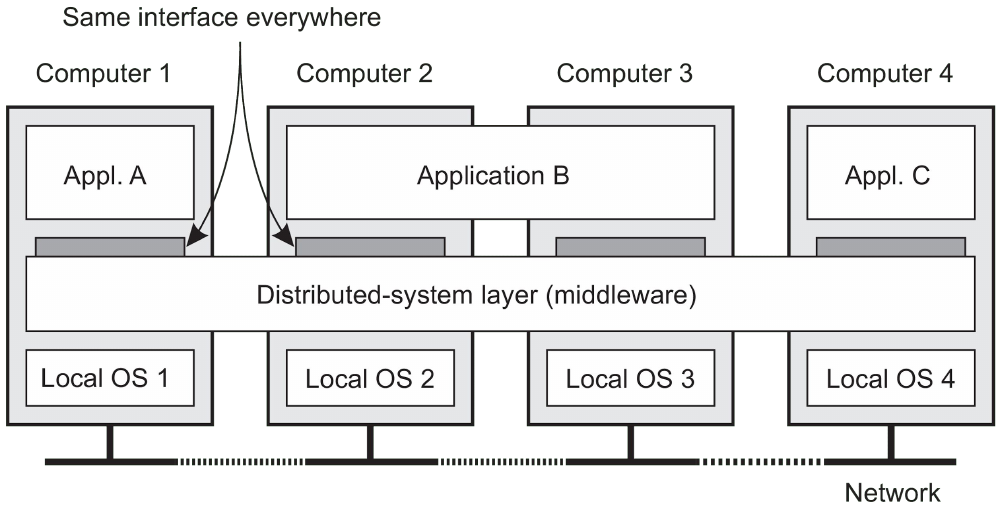
\includegraphics[scale=0.50]{img/middle.png}
				\caption{Middleware layer}
			\end{figure}
			Il \textbf{middleware} è un insieme di applicazioni e protocolli "\textbf{general purpose}" che risiedono all'interno del livello applicativo. è dunque un livello software che astrae dall'eterogeneità di rete, hardware, sistemi operativi e linguaggi di programmazione, con lo \textbf{scopo di fornire interfacce comuni che assicurino  modelli di comunicazione e di computazione uniformi}.  Questo livello, dunque, costituisce un insieme di protocolli condivisi dalle applicazioni più specifiche al livello soprastante.
			In sintesi, un livello middleware offre servizi alle applicazioni quali:
			\begin{itemize}
				\item Comunicazione;
				\item Meccanismi di sicurezza;
				\item Transazioni
				\item Error-recovery;
				\item Gestione di risorse condivise.
			\end{itemize}
			\textbf{Questi servizi sono indipendenti rispetto alle specifiche applicazioni.} 
			Alcuni esempi:
			\begin{itemize}
				\item Protocolli di autenticazione e autorizzazione (criptografia ssh)
				\item Protocolli di commit. Sono utilizzati per realizzare l'atomicità nelle transazioni. Stabiliscono se in un insieme di processi tutti hanno svolto una particolare operazione o se non è stata svolta affatto.
			\end{itemize}
			Nello specifico vedremo come i \textbf{protocolli di comunicazione middleware supportino servizi di comunicazione ad alto livello} e permettano, per esempio, la chiamata a procedure o oggetti remoti in modo \textbf{trasparente.}
			 
		\subsubsection{Coordinazione diretta}
				
			Un tipi di comunicazione nella quale le componenti partecipanti sono:
			\begin{itemize}
				\item \textbf{Referentially coupled}: durante la comunicazione gli attori utilizzano riferimenti espliciti ai loro interlocutori.
				\item \textbf{Temporally coupled}: entrambe le componenti devono essere in esecuzione (up and running).	
			\end{itemize}
			Il libro propone un'introduzione ai tipi di comunicazione (persist, transient, synchronous, asynchronous).
			
	\subsection{Remote Procedure Call}
		Molti sistemi distribuiti sono basati sullo scambio di messaggi tra processi, tuttavia questo tipo di approccio non permette di nascondere la comunicazione tra le componenti in modo da rendere trasparente il contesto distribuito. \\
		Una soluzione al problema è stata proposta da Nelson e Birrell (1984) introducendo una modalità completamente differente nella gestione della comunicazione nel contesto di un sistema distribuito.
		In breve la proposta è quella di chiamare procedure che sono localizzate su macchine remote:
		\begin{enumerate}
			\item quando A chiama B il processo chiamante in A è sospeso;
			\item l'esecuzione della procedura chiamata ha luogo in B;
			\item A invia i parametri della chiamata a B che a sua volta risponderà con il risultato della chiamata;
			\item \textbf{Nessun passaggio di messaggi è visibile dal punto di vista del programmatore.}
		\end{enumerate}
		La soluzione ha le seguenti problematiche:
		\begin{itemize}
			\item le procedure chiamante e chiamato si trovano su macchine diverse e non condividono lo stesso address space;
			\item la rappresentazione dei parametri e del risultato di ritorno può differire sulle macchine interessate;
			\item Le due macchine potrebbero crashare.
		\end{itemize}
		
		
		
				
			
				
				
			
		
		
		
		
		
		
		
		
		
		
		
		
		
		
		
		
		
		
		
		
		
		
		
		
		
		
		
		

\end{document}